\documentclass[11pt,a4paper]{article}
\usepackage[T1]{fontenc}
\usepackage[margin=2.3cm]{geometry}
\usepackage{amsmath,amssymb}
\usepackage{graphicx}
\usepackage[dvipsnames]{xcolor}
\usepackage{enumitem}
\usepackage[colorlinks=true,linkcolor=blue,urlcolor=blue]{hyperref}
\setlength{\parskip}{0.6em}
\setlength{\parindent}{0pt}
\begin{document}

\begin{center}{\LARGE\bfseries openseismo}\\[0.4em]{\large Locate an earthquake from seismograph arrivals, in three sessions.}\\[0.2em]\small PAN IIT OSS explainer \textbullet{} secondary school to diploma / undergraduate (levels 3-5)\end{center}

\section*{Why this exists}
When an earthquake happens, waves of two kinds travel through the ground at different speeds. This explainer shows how the gap between their arrivals gives distance, how several stations give position, and how least squares copes with noisy arrival times.

\section*{The end goal}
Locate an earthquake from seismograph arrivals. The end goal is to locate an earthquake from seismograph arrivals, with an honest error ellipse. The same least-squares idea is used for GPS, lightning detection and sound-source localisation. This material is for learning only: it cannot predict earthquakes or warn anyone.

\section*{How the three sessions build up}
\begin{enumerate}[nosep]
\item \textbf{Session 1: Two waves, one gap: how far away was it?} (Level 1, conceptual interactive model, 60 min).
\item \textbf{Session 2: Three circles pin down the epicentre} (Level 2, mathematical engineering model, 75 min).
\item \textbf{Session 3: Real-world location: Geiger's method, pick errors and geometry} (Level 3, simulation and validation, 90 min).
\end{enumerate}

\section{Session 1: Two waves, one gap: how far away was it?}

\subsection*{A. Real-world problem}
During a storm you see lightning and count the seconds until the thunder: the longer the wait, the farther away the strike. An earthquake works the same way, but both signals are waves in the ground. The first to arrive is the P wave (fast, a push-pull squeeze along the direction of travel); later comes the S wave (slower, a side-to-side shake). A seismograph records both. Can the wait between them tell you how far away the earthquake was? This repo is for learning only: it cannot warn anyone, and earthquakes cannot be predicted.

\subsection*{B. Concept and theory}
A wave covering a distance d at speed v needs the time t = d / v. In typical upper crust we use vp = 6.0 km/s for P waves and vs = 3.5 km/s for S waves (approximate teaching values; real rock varies from place to place). Both start together at the quake, so the S wave falls behind: after distance d the gap is gap = d / vs - d / vp. Turning this around gives d = gap x vp x vs / (vp - vs). With our speeds each second of gap is worth 6.0 x 3.5 / 2.5 = 8.4 km. The lightning rule is the same idea with light (instant) in place of P and sound (about 343 m/s, so 2.9 s per kilometre) in place of S.

\begin{itemize}[nosep]
\item d: distance from the quake to the station (km)
\item vp: P wave speed (approximate typical value 6.0) (km/s)
\item vs: S wave speed (approximate typical value 3.5) (km/s)
\item tp, ts: arrival time of P and S, measured from the start of the quake (s)
\item gap: S-P gap = ts - tp (s)
\end{itemize}

\begin{equation*}
t=\frac{d}{v}
\end{equation*}

\begin{equation*}
\text{gap}=t_s-t_p=\frac{d}{v_s}-\frac{d}{v_p}
\end{equation*}

\begin{equation*}
d=\text{gap}\cdot\frac{v_p v_s}{v_p-v_s}\qquad \frac{v_p v_s}{v_p-v_s}=8.4\ \text{km/s}
\end{equation*}

\begin{center}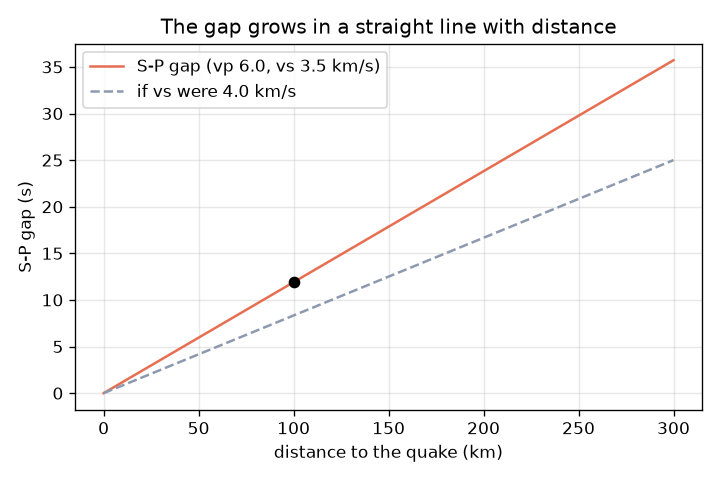
\includegraphics[width=0.85\linewidth]{figures/s01_gap_vs_distance.png}\\\small The S-P gap grows in a straight line with distance (35.7 s at 300 km).\end{center}

\subsection*{E. Worked example}
A station is 100 km from a quake. Find the P and S arrival times and the gap, then recover the distance from the gap.
\begin{enumerate}[nosep]
\item P wave: tp = 100 / 6.0 = 16.7 s.
\item S wave: ts = 100 / 3.5 = 28.6 s.
\item Gap = 28.6 - 16.7 = 11.9 s (11.905 before rounding).
\item Rule: 1 s of gap = 6.0 x 3.5 / (6.0 - 3.5) = 8.4 km.
\item Distance = 11.905 x 8.4 = 100 km. The round trip agrees.
\end{enumerate}
\textbf{Answer.} P at 16.7 s, S at 28.6 s, gap 11.9 s, which gives back 100 km.

\subsection*{F. Questions}
\begin{enumerate}[nosep]
\item \textbf{Conceptual.} Why does the P wave always arrive before the S wave? What would the seismogram look like if the quake were very close to the station?
\item \textbf{Numerical.} A station reads an S-P gap of 15 s. How far away was the quake? Check that the answer is reasonable.
\item \textbf{Graph and simulation interpretation.} On the gap-versus-distance graph, what is the gap at 300 km? What does the slope of the line mean? What changes if the S speed rises to 4.0 km/s?
\item \textbf{Design and optimisation challenge.} Design: a seismograph clock can be wrong by up to 0.5 s in the S-P gap you read. How much distance error does that cause, and is it acceptable for a regional map where you want to be within 10 km?
\end{enumerate}

\section{Session 2: Three circles pin down the epicentre}

\subsection*{A. Real-world problem}
One station tells you only how far away a quake was, not where. Seismologists use several stations. Three stations at known positions each give a distance; where the three circles meet is the epicentre. How many stations do you really need, how do you compute the meeting point, and how badly does a timing error move it? (Opengps uses the same circle idea with satellites; this session is the earthquake version. Openemwave and openoscillator cover waves in general.)

\subsection*{B. Concept and theory}
In an ideal uniform elastic solid the wave speeds depend on how the material resists compression and shear. Their ratio depends only on Poisson's ratio nu: vp / vs = sqrt(2 (1 - nu) / (1 - 2 nu)). For nu = 0.25 this is sqrt(3) = 1.732; our approximate 6.0 / 3.5 = 1.714 corresponds to nu = 0.242, so the numbers are consistent, though real rock only roughly follows an ideal solid. At each station the origin time cancels in the S-P gap, so d = (ts - tp) vp vs / (vp - vs). A station i at (xi, yi) with distance ri puts the epicentre on a circle (x - xi)\textasciicircum{}2 + (y - yi)\textasciicircum{}2 = ri\textasciicircum{}2. Subtracting the first station's circle from the others removes x\textasciicircum{}2 + y\textasciicircum{}2 and leaves straight lines, 2 (xi - x1) x + 2 (yi - y1) y = r1\textasciicircum{}2 - ri\textasciicircum{}2 + xi\textasciicircum{}2 + yi\textasciicircum{}2 - x1\textasciicircum{}2 - y1\textasciicircum{}2, which are solved for (x, y). Two circles meet in two points (a point and its mirror image across the line joining the stations); the third station picks the right one. If the three stations lie on one line, the lines are parallel and no unique answer exists.

\begin{itemize}[nosep]
\item nu: Poisson's ratio of the rock (no unit)
\item (xi, yi): position of station i on a flat map (km)
\item ri: distance from station i to the epicentre (km)
\item (x, y): unknown epicentre position (km)
\item ts, tp: S and P arrival times (s)
\end{itemize}

\begin{equation*}
\frac{v_p}{v_s}=\sqrt{\frac{2(1-\nu)}{1-2\nu}}\;\xrightarrow{\nu=0.25}\;\sqrt3
\end{equation*}

\begin{equation*}
d=(t_s-t_p)\frac{v_p v_s}{v_p-v_s}
\end{equation*}

\begin{equation*}
(x-x_i)^2+(y-y_i)^2=r_i^2
\end{equation*}

\begin{equation*}
2(x_i-x_1)\,x+2(y_i-y_1)\,y=r_1^2-r_i^2+x_i^2+y_i^2-x_1^2-y_1^2
\end{equation*}

\begin{center}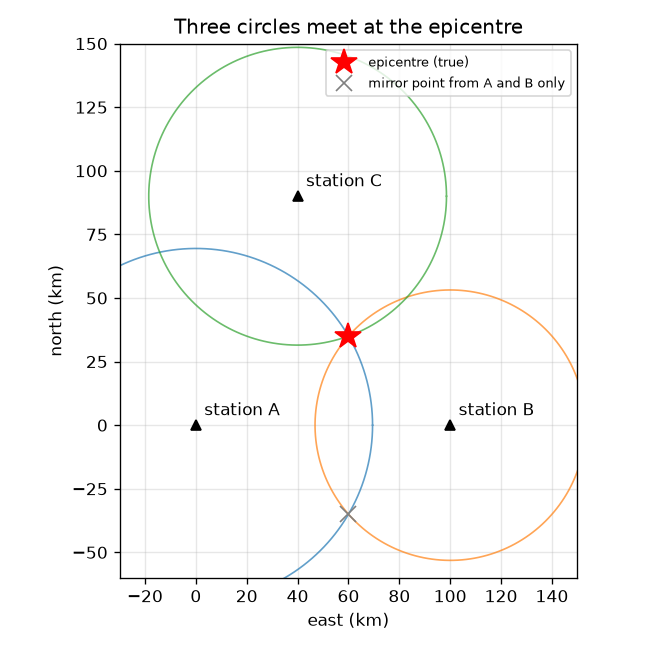
\includegraphics[width=0.85\linewidth]{figures/s02_three_circles.png}\\\small Three circles meet at the epicentre (60, 35) km; A and B alone also meet at the mirror point.\end{center}

\subsection*{E. Worked example}
Stations A (0, 0), B (100, 0), C (40, 90) km record a quake at (60, 35) km. Compute the distances and S-P gaps, then recover the epicentre from the gaps.
\begin{enumerate}[nosep]
\item Distances: rA = sqrt(60\textasciicircum{}2 + 35\textasciicircum{}2) = 69.46 km, rB = sqrt(40\textasciicircum{}2 + 35\textasciicircum{}2) = 53.15 km, rC = sqrt(20\textasciicircum{}2 + 55\textasciicircum{}2) = 58.52 km.
\item Gaps: rA / 8.4 = 8.27 s, rB / 8.4 = 6.33 s, rC / 8.4 = 6.97 s. Going back, 8.27 x 8.4 = 69.5 km.
\item Line from A and B: 200 x = rA\textasciicircum{}2 - rB\textasciicircum{}2 + 100\textasciicircum{}2 = 12000, so x = 60 km.
\item Line from A and C: 80 x + 180 y = rA\textasciicircum{}2 - rC\textasciicircum{}2 + 40\textasciicircum{}2 + 90\textasciicircum{}2 = 11100. With x = 60: 180 y = 6300, so y = 35 km.
\item The epicentre is (60, 35) km. Check: the mirror point (60, -35) is 126.6 km from C, not 58.5 km.
\end{enumerate}
\textbf{Answer.} Epicentre (60, 35) km, recovered exactly from the three S-P gaps (8.27, 6.33 and 6.97 s).

\subsection*{F. Questions}
\begin{enumerate}[nosep]
\item \textbf{Conceptual.} Why do two stations leave two possible epicentres, and why does a third station fix this? Why do three stations on one straight line still fail?
\item \textbf{Numerical.} Compute the ratio vp/vs for Poisson's ratio 0.25 and compare it with 6.0 / 3.5. Which Poisson's ratio gives exactly 6.0 / 3.5?
\item \textbf{Graph and simulation interpretation.} In the app, set the quake to (60, 35) km and add a clock error of +1.0 s at station A. Describe how the black dot moves relative to the red cross. Is the error the same everywhere on the map?
\item \textbf{Design and optimisation challenge.} Design: you can place a third station at (50, 0), (100, 90) or (40, 90) next to A (0, 0) and B (100, 0). Which choices let you find an epicentre at (60, 35) km, and which fail? What is the minimum number of stations for an epicentre from S-P times, and why?
\end{enumerate}

\section{Session 3: Real-world location: Geiger's method, pick errors and geometry}

\subsection*{A. Real-world problem}
In real life nobody tells you when the quake started, and arrival times are picked by eye or by software with errors of a fraction of a second. So you have three unknowns (east x, north y and origin time t0) and several noisy P arrival times. How do you find the best epicentre, how wrong can it be, which networks are good, and what happens if the speed model is wrong? Remember: this only locates a quake after it happened; it is not a warning or prediction tool, and earthquakes cannot be predicted.

\subsection*{B. Concept and theory}
At station i the P wave arrives at ti = t0 + Ri / vp with Ri = sqrt((xi - x)\textasciicircum{}2 + (yi - y)\textasciicircum{}2). The unknowns (x, y, t0) enter non-linearly, so Geiger's method guesses, linearises and repeats: with residual ri = observed - predicted, a small change dm = (dx, dy, dt0) changes ti by Ji . dm where Ji = (-(xi - x)/(vp Ri), -(yi - y)/(vp Ri), 1). Solve J dm = r in the least-squares sense, add dm to the guess, and iterate (Gauss-Newton). If picks have independent Gaussian errors of standard deviation sigma, the solution has covariance C = sigma\textasciicircum{}2 (J\textasciicircum{}T J)\textasciicircum{}-1; its (x, y) block gives the 95 percent error ellipse with semi-axes sqrt(5.991 lambda), where lambda are the eigenvalues and 5.991 is the 95 percent point of the chi-square distribution with 2 degrees of freedom. Two numbers summarise geometry: the condition number of J (large means nearly degenerate) and the horizontal dilution sqrt(Cxx + Cyy)/sigma in km per second of pick error. The failure case is a two-layer Earth (thickness H over a faster half-space, speeds v1 \textless{} v2): the first arrival is the direct wave x / v1 or the head wave x / v2 + 2H sqrt(v2\textasciicircum{}2 - v1\textasciicircum{}2)/(v1 v2), whichever is earlier, so the travel-time curve has a kink and no single constant speed fits. For magnitude we use the approximate educational formula ML = log10 A + 3 log10(8 dt) - 2.92, where A is the peak amplitude in mm on a Wood-Anderson seismograph and dt the S-P time in seconds (a textbook form; agencies use calibrated scales).

\begin{itemize}[nosep]
\item (x, y): unknown epicentre (km)
\item t0: unknown origin time (s)
\item ti: observed P arrival at station i (s)
\item sigma: standard deviation of a pick error (s)
\item J: Jacobian: change of arrival time per change of (x, y, t0) (s/km, s/km, no unit)
\item C: covariance of the solution (km\textasciicircum{}2, km\textasciicircum{}2 (and s\textasciicircum{}2))
\item H, v1, v2: layer thickness and speeds of the toy Earth (15 km, 5.0 and 7.0 km/s) (km, km/s)
\item A, dt, ML: amplitude in mm, S-P time in s, magnitude (mm, s, no unit)
\end{itemize}

\begin{equation*}
t_i=t_0+\frac{R_i}{v_p},\quad R_i=\sqrt{(x_i-x)^2+(y_i-y)^2}
\end{equation*}

\begin{equation*}
J_i=\left(-\frac{x_i-x}{v_pR_i},\,-\frac{y_i-y}{v_pR_i},\,1\right),\qquad J\,\delta m=r\;\Rightarrow\;\delta m=(J^{\mathsf T}J)^{-1}J^{\mathsf T}r
\end{equation*}

\begin{equation*}
C=\sigma^2\,(J^{\mathsf T}J)^{-1},\qquad a_{95},\,b_{95}=\sqrt{5.991\,\lambda_{1,2}}
\end{equation*}

\begin{equation*}
t_{\text{head}}=\frac{x}{v_2}+\frac{2H\sqrt{v_2^2-v_1^2}}{v_1v_2}
\end{equation*}

\begin{equation*}
M_L=\log_{10}A+3\log_{10}(8\,\Delta t)-2.92
\end{equation*}

\begin{center}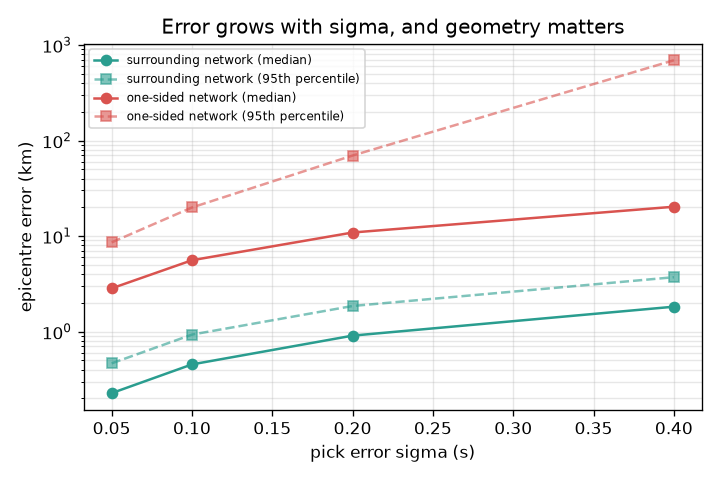
\includegraphics[width=0.85\linewidth]{figures/s03_error_vs_sigma.png}\\\small Epicentre error against pick noise: proportional to sigma, and strongly dependent on station geometry.\end{center}

\subsection*{E. Worked example}
For the surrounding network, quake (55, 40) km, vp = 6.0 km/s: compute the Jacobian row of station (5, 10) at the true quake, then describe the first Gauss-Newton step from the station centroid (50, 53).
\begin{enumerate}[nosep]
\item Distance R = sqrt(50\textasciicircum{}2 + 30\textasciicircum{}2) = 58.31 km.
\item Jx = -(5 - 55) / (6.0 x 58.31) = 50 / 349.9 = 0.143 s/km.
\item Jy = -(10 - 40) / (6.0 x 58.31) = 30 / 349.9 = 0.086 s/km, and Jt0 = 1.
\item The start (50, 53) is sqrt(5\textasciicircum{}2 + 13\textasciicircum{}2) = 13.9 km from the truth.
\item One step with all five rows reduces that to 0.21 km, and the next step to essentially zero (noise-free picks).
\end{enumerate}
\textbf{Answer.} Jacobian row (0.143, 0.086, 1); the iteration starts 13.9 km away and is within 0.21 km after one step.

\subsection*{F. Questions}
\begin{enumerate}[nosep]
\item \textbf{Conceptual.} Why do stations all on one side of the quake give a much worse epicentre than stations all around it, even with the same pick errors?
\item \textbf{Numerical.} A station with S-P gap 20 s records a peak amplitude of 2 mm. Estimate ML with the approximate formula. Is it plausible? How does ML change for 20 mm?
\item \textbf{Graph and simulation interpretation.} In the error-versus-sigma figure, what is the median error of the surrounding network at sigma = 0.2 s, and for the one-sided network? What does a straight line on the log plot tell you?
\item \textbf{Design and optimisation challenge.} Design: you must report epicentres within about 1.5 km (95 percent) using picks with sigma = 0.1 s. Would the surrounding network meet this? What about the one-sided network, and what is the cheapest fix for it?
\end{enumerate}

\section{Real-world mini-project}
\textbf{Locate a synthetic quake from five noisy stations.} A synthetic earthquake (true epicentre (55, 40) km, origin time 3 s) is recorded by the five surrounding stations of Session 3, at vp = 6.0 km/s. Add Gaussian noise of 0.1 s to the P picks (random seed 3), locate the quake with \texttt{geiger}, report the epicentre error in km, and draw the 95 percent error ellipse from the covariance. Then repeat with the one-sided network and compare.

\section{The path ahead}
\begin{enumerate}[nosep]
\item \textbf{Session 4: Survive a bad pick.} A location routine that spots and drops (or down-weights) a blunder in one pick.
\item \textbf{Session 5: Fix the network.} A tool that suggests where to put one more station.
\item \textbf{Session 6: Use the layers.} A locator that predicts first arrivals with the two-layer model instead of one speed.
\item \textbf{Session 7: Add depth.} A four-unknown locator (x, y, depth, t0) with a vertical error bar.
\item \textbf{Session 8: Reproduce the Target animation.} A GIF of expanding P and S wavefronts, per-station seismograms with picks and the iteration path.
\end{enumerate}

\section{Answers and hints}

\subsection*{Session 1}
\begin{enumerate}[nosep]
\item \textbf{Conceptual.} Hint: Which wave has the higher speed? What happens to the gap as the distance gets smaller? Solution: P is faster (6.0 against 3.5 km/s in our model), so over any distance it needs less time. The gap is proportional to distance, so for a very close quake the gap is tiny and the P and S wiggles run into each other; the two arrivals are hard to separate by eye.
\item \textbf{Numerical.} Hint: Use 1 s of gap = 8.4 km. Solution: Distance = 15 x 8.4 = 126 km. Check: P needs 126 / 6.0 = 21.0 s and S needs 126 / 3.5 = 36.0 s, a gap of 15.0 s. The result is in kilometres and is a sensible regional distance.
\item \textbf{Graph and simulation interpretation.} Hint: Slope = gap / distance = 1/vs - 1/vp. Solution: At 300 km the gap is 35.7 s. The slope, 1/3.5 - 1/6.0 = 0.119 s per km, is the extra delay of S per kilometre travelled (equivalently 1 s per 8.4 km). A faster S wave makes the line flatter: at 100 km the gap would be 8.33 s instead of 11.9 s, so the same measured gap would mean a larger distance.
\item \textbf{Design and optimisation challenge.} Hint: Multiply the timing error by km per second of gap. Solution: 0.5 s x 8.4 km/s = 4.2 km. That is inside a 10 km budget, but a single station still gives only a distance (a circle), not a position, and the speeds themselves are uncertain by several percent, so the real error is larger. Trade-off: a faster sampling rate and careful picking cut the timing error; a second and third station are needed for direction (Session 2).
\end{enumerate}

\subsection*{Session 2}
\begin{enumerate}[nosep]
\item \textbf{Conceptual.} Hint: Draw two circles that overlap. Where does the third circle have to go? Solution: Two circles centred on different points meet in two points that are mirror images across the line joining the centres. A third station not on that line has a circle that passes through only one of the two points, so it picks the right one. If all three stations are on one line, every circle is mirror-symmetric about that line, so the mirror point fits all of them: the answer stays ambiguous (and the linear system has rank 1, so the code rejects it).
\item \textbf{Numerical.} Hint: Use vp/vs = sqrt(2 (1 - nu) / (1 - 2 nu)); to invert, square the ratio first: nu = (q - 2) / (2 (q - 1)) with q = (vp/vs)\textasciicircum{}2. Solution: nu = 0.25 gives sqrt(2 x 0.75 / 0.5) = sqrt(3) = 1.732. And 6.0 / 3.5 = 1.714, a 1 percent difference. For q = 1.714\textasciicircum{}2 = 2.939 we get nu = 0.939 / (2 x 1.939) = 0.242. Both values are typical of crustal rock.
\item \textbf{Graph and simulation interpretation.} Hint: Move the quake to (10, 10) and compare. Solution: The estimate lands 7.4 km away from the true point at (60, 35), because circle A grows by 8.4 km. At (10, 10), close to station A, the same 1.0 s clock error moves the estimate by only 1.9 km. The effect of a timing error depends on where the quake is relative to the network.
\item \textbf{Design and optimisation challenge.} Hint: A station on the line through A and B adds no new information about north-south position. Solution: (50, 0) is on the line through A and B: the system is rank deficient and the code refuses it. (100, 90) and (40, 90) are both off the line and work; (40, 90) is the choice we used. Three non-collinear stations are the minimum, because two circles leave a mirror ambiguity. A fourth station gives a check and lets you average out errors. Trade-off: more stations cost more, but protect against one bad reading.
\end{enumerate}

\subsection*{Session 3}
\begin{enumerate}[nosep]
\item \textbf{Conceptual.} Hint: Think about the directions from the quake to the stations, and what the columns of J look like when those directions are nearly equal. Solution: The x and y columns of J are the directions to the stations divided by vp. If the stations all lie in nearly the same direction, those columns become nearly parallel to each other and to the constant t0 column, so J is nearly degenerate (condition number 195 against 9.2) and a small timing change can slide the solution a long way along the line of sight (horizontal dilution 85 km/s against 5.5 km/s). With stations all around, the directions cancel and the solution is stiff.
\item \textbf{Numerical.} Hint: ML = log10 A + 3 log10(8 dt) - 2.92. Solution: log10(2) = 0.301; 8 x 20 = 160, log10(160) = 2.204, times 3 = 6.612; ML = 0.301 + 6.612 - 2.92 = 3.99, about 4.0 (approximate). Ten times the amplitude adds exactly 1.0 to ML, so 20 mm gives about 5.0. Sanity check: a magnitude near 4 at about 170 km (20 s x 8.4 km/s = 168 km) with a few mm of motion is plausible.
\item \textbf{Graph and simulation interpretation.} Hint: Compare 0.2 s with 0.1 s: doubling sigma. Solution: At sigma = 0.2 s the surrounding network has a median error of 0.91 km and the one-sided network 10.9 km, roughly twelve times worse. A rising line means the error grows with sigma: doubling sigma doubles the error (0.45 km at 0.1 s, 0.91 km at 0.2 s), as linear theory says. Geometry sets the proportionality constant. The 95th percentile of the one-sided network is even worse because the iteration can diverge for unlucky noise.
\item \textbf{Design and optimisation challenge.} Hint: Use the ellipse semi-axes and the dilution numbers. Solution: The surrounding network has a 95 percent ellipse of about 1.0 x 0.9 km, so yes. The one-sided network has a median error of 5.6 km and 95th percentile near 20 km: no. A cheap fix is one extra station on the far side: a station at (100, 90) km cuts the horizontal dilution from 85 km/s to below 12 km/s. The alternative, better picks, costs more effort and helps only in proportion to sigma. Remember also the layered-Earth bias, which no number of stations removes while the speed model is wrong.
\end{enumerate}

\section{How to join}
Read \texttt{CONTRIBUTING.md} in the repository, then pick an issue labelled \texttt{good first issue}. Repository: \url{https://github.com/KrunalPanchal1995/openseismo}

\end{document}
